\documentclass[conference]{IEEEtran}
\IEEEoverridecommandlockouts
\usepackage{cite}
\usepackage{amsmath,amssymb}
\usepackage{graphicx}
\usepackage{booktabs}
\usepackage{xcolor}
\usepackage{url}
\usepackage[hidelinks]{hyperref}

\newcommand{\ours}{Faithful Seam Carving}
\newcommand{\best}[1]{\textbf{#1}}

\begin{document}

\title{Faithful Seam Carving: Measuring and Preventing\\Object Destruction and Fusion in Content-Aware Resizing}

\author{\IEEEauthorblockN{Aayush Kapoor, Riya Saitwal, Poorav Parekh}
\IEEEauthorblockA{Department of Computer Engineering, NMIMS [Campus], India\\
\relax [email addresses]}}

\maketitle

\begin{abstract}
Seam carving resizes an image by repeatedly deleting the cheapest connected path of pixels. Its cost is defined on pixels, not objects, so it can delete most of an object or remove the background between two objects until they merge. Viewers penalise these failures heavily, yet no standard retargeting metric counts them. We make three contributions. First, an object-level evaluation protocol that uses exact pixel correspondences to count objects that are crushed, vanished or fused, and that scores the detail of each object by comparing it with itself. Second, an ablation of 18 configurations on 413 annotated objects in 70 COCO images. It shows that classical fixes do not protect objects: line and saliency protection lower the share of intact objects at half width from 64.9\% to 48.7\% and 57.4\%, and static object masks trade crushing for fusion (41.4\% of objects fused). Third, \ours{}, a training-free method that protects thin gaps between neighbouring objects and adds an exact integrity guard that stops carving before a seam harms any object; uniform scaling completes the resize. At half width it keeps 99.0\% of objects intact (plain seam carving: 64.9\%) and improves on uniform scaling in both per-object detail (0.911 vs.\ 0.865 SSIM) and aspect distortion (0.464 vs.\ 0.693), at 0.53\,s per image.
\end{abstract}

\begin{IEEEkeywords}
image retargeting, seam carving, content-aware resizing, object integrity, evaluation metrics
\end{IEEEkeywords}

\section{Introduction}

Changing the aspect ratio of a photograph forces a choice. Cropping discards content at the borders, and uniform scaling keeps everything but squashes it. Seam carving~\cite{avidan2007seam} offers a third option: it repeatedly removes a connected path of low-energy pixels (a \emph{seam}), so that flat background is removed first and textured content is kept.

The energy that guides seam carving is a property of pixels, such as the local gradient, not of objects. Nothing prevents seams from passing through an object once the cheaper background has been used up, and once a cheap path through an object exists, neighbouring paths tend to be cheap as well, so seams concentrate and \emph{crush} it. Seams also remove the background strip between two objects until the objects touch, \emph{fusing} them into one shape. In the RetargetMe study~\cite{rubinstein2010comparative}, 210 participants compared eight retargeting methods in pairs on 37 images of an 80-image benchmark; plain seam carving ranked last overall, and its rejections were dominated by distorted lines and deformed people and objects. The same study found that most automatic retargeting metrics are not consistent with human rankings. To our knowledge, no metric in this literature counts how many objects survive a resize.

\begin{figure*}[t]
\centering
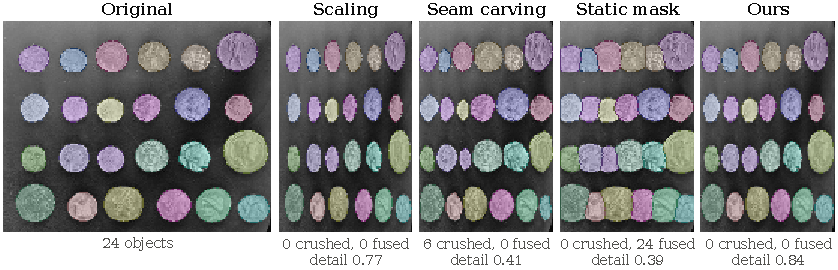
\includegraphics[width=\textwidth]{figs/coins.pdf}
\caption{The 24 coins of the scikit-image \emph{coins} photo resized to half width. Each object keeps its own tint before and after, so crushed and fused coins are easy to spot. Plain seam carving crushes 6 coins; a static mask protects them but fuses 24 coins into 20 touching pairs; \ours{} keeps every coin separate and keeps more detail than scaling (0.84 vs.\ 0.77). Coins are segmented by watershed; carving does 34\% of the resize.}
\label{fig:coins}
\end{figure*}

This paper treats object integrity as the primary quantity to measure and to protect. Our contributions are:
\begin{enumerate}
\item \textbf{Object-integrity evaluation.} Every method we test returns, for each output pixel, the input pixel it came from. From this map we count objects that are \emph{crushed} (more than half of their pixels deleted), \emph{vanished}, \emph{fused} (touching another object they did not touch before) or \emph{worse than scaling}, and we score \emph{per-object detail} as the SSIM between each object and its own resized output.
\item \textbf{A systematic ablation.} On 413 ground-truth objects in 70 COCO images, we evaluate 18 configurations, including three classical fixes (line protection, saliency, an early stop) and static object masks. Two of the classical fixes reduce integrity, and static masks replace crushing with fusion.
\item \textbf{\ours{}.} A per-object cost budget, protection of thin gaps between objects, and an exact integrity guard with a single dial. With the dial at zero, seams remove only background that does not bring objects into contact, and scaling finishes the resize. This keeps 99.0\% of objects intact at half width and keeps more object detail, with less squash, than uniform scaling.
\end{enumerate}
The method needs no training and runs on a CPU. Our implementation, tests and all experiment scripts are available at \url{https://github.com/Aayush-K15/faithful-seam-carving}.

\section{Related Work}

\textbf{Seam carving and its energy.} Avidan and Shamir~\cite{avidan2007seam} introduced seam carving with a gradient (``backward'') energy, dynamic-programming seam search, seam insertion for enlarging, and object removal with user-painted masks. Rubinstein et al.~\cite{rubinstein2008improved} proposed \emph{forward energy}, which charges a seam for the new edges it creates, and extended carving to video with graph cuts. Later work added saliency~\cite{achanta2009saliency} and edge or line preservation~\cite{kiess2010edge} to the energy. All of these protect pixels with high cost; none guarantees that an object survives.

\textbf{Combining operators.} Dong et al.~\cite{dong2009optimized} observed that carving all the way creates artefacts and proposed carving part of the way and scaling the rest, choosing the switch point with a whole-image distance. Multi-operator retargeting~\cite{rubinstein2009multiop} searches over sequences of cropping, scaling and carving. Our guard also stops carving and scales the remainder, but its trigger is exact, per-object damage rather than global similarity, which can stay low while a small object is lost.

\textbf{Objects in retargeting.} Dong et al.~\cite{dong2014summarization} deliberately remove repeated objects to save space, showing that changing the object count is a real effect of retargeting. Scene carving~\cite{mansfield2010scene} uses user-supplied depth layers. Dickman and Diefenbach~\cite{dickman2024directorial} turn text prompts into CLIPSeg masks that weight the seam energy; this is a static mask in our terminology, and it reports no quantitative evaluation of object damage.

\textbf{Learning-based retargeting.} Cho et al.~\cite{cho2017weakly} learn where to shrink with a network. Prune and Repaint~\cite{shen2024prune} prunes columns by importance and repaints damaged regions with a diffusion model. Elsner et al.~\cite{elsner2024deformation} learn continuous deformation fields that also apply to 3D data. These methods need trained models, and none provides a guarantee on object integrity. Our metrics apply to their outputs unchanged.

\section{Background: Seam Carving with Forward Energy}

For a grey image $I$ of size $H\times W$, a vertical seam is a path $\{(i, s_i)\}_{i=1}^{H}$ with $|s_i - s_{i-1}|\le 1$. With forward energy~\cite{rubinstein2008improved}, removing pixel $(i,j)$ creates new neighbours, and the cost of the new edges depends on which parent the seam came from:
\begin{align}
C_U(i,j) &= |I(i,j{+}1) - I(i,j{-}1)|,\nonumber\\
C_L(i,j) &= C_U(i,j) + |I(i{-}1,j) - I(i,j{-}1)|,\\
C_R(i,j) &= C_U(i,j) + |I(i{-}1,j) - I(i,j{+}1)|.\nonumber
\end{align}
The cumulative cost is computed by dynamic programming,
\begin{equation}
M(i,j) = P(i,j) + \min\begin{cases}
M(i{-}1,j{-}1) + C_L(i,j)\\
M(i{-}1,j) + C_U(i,j)\\
M(i{-}1,j{+}1) + C_R(i,j),
\end{cases}
\end{equation}
where $P$ is an optional extra cost per pixel (zero for plain carving). The cheapest seam is recovered by backtracking from the minimum of the last row in $O(HW)$ time. We clamp the image at its borders, so that the outermost columns are not free to remove. Horizontal seams are found on the transposed image. Our engine records, for every output pixel, its source row and column in the input; every method in this paper, including scaling and cropping, returns this map.

\section{Method}

\ours{} takes an instance label map $L$ (0 for background, $1,\dots,N$ for objects), from ground truth or from a segmentation model. Before each seam it builds the extra cost $P$ from two terms, and before removing the seam it applies a guard.

\subsection{Per-object budget}
A static mask gives every object pixel the same extra cost. Once background runs out, a static mask does not distinguish an untouched object from one that has already lost most of its pixels, so seams can return to the same object. We make the cost grow with the damage already done. Let $A_k^0$ be the area of object $k$ in the input and $A_k$ its area in the current, partially carved image, and let $d_k = 1 - A_k/A_k^0$. Every pixel of object $k$ receives
\begin{equation}
P_{\text{obj}}(p) = \lambda\, e^{\gamma d_k}, \qquad p \in \text{object } k.
\end{equation}
With $\gamma = 0$ this is the static mask. We use $\lambda=1$ and $\gamma=8$, so the cost is about $2.2\lambda$ when 10\% of an object is gone and about $55\lambda$ at 50\%.

\subsection{Gap protection}
The budget alone stops crushing but not fusion: seams are pushed into the narrow background strips between objects. A vertical seam removes one pixel from every row, so it narrows horizontal gaps. We mark a background pixel as a \emph{gap pixel} if, along its row, it lies in a background run of at most $g$ pixels whose two ends are pixels of two \emph{different} objects (along columns for horizontal seams), and add $\mu$ to its cost:
\begin{equation}
P(p) = P_{\text{obj}}(p) + \mu\,[p \in \text{gap}_g].
\end{equation}
We use $g = 3$\,px and $\mu = 50$. Wider background stays free to carve.

\subsection{Integrity guard and the dial}
Costs make damage unlikely but cannot rule it out: when no cheap seam remains, the cheapest one may still cross an object. Before a seam is removed, the guard computes its exact effect. It counts the pixels of each object on the seam and refuses the seam if any object would have lost more than a fraction $\tau$ of its original pixels. It also removes the seam from the label map and refuses it if two objects that were not 4-adjacent in the input would become 4-adjacent. On refusal, carving stops and the remaining size change is done by uniform scaling (or, optionally, by an object-aware crop).

The threshold $\tau$ is a dial. At $\tau=0.5$ every object survives as a separate shape, but seams still run through objects and deform them. At $\tau=0$, the default, seams may remove only background, and carving stops at the first seam that would touch an object or close a gap. Because no object then loses pixels, $d_k$ stays 0 and the budget reduces to a static mask; the budget matters for $\tau > 0$. The guard costs $O(HW)$ per seam, the same order as the seam search, so carving $k$ seams costs $O(kHW)$ in total.

\begin{figure*}[t]
\centering
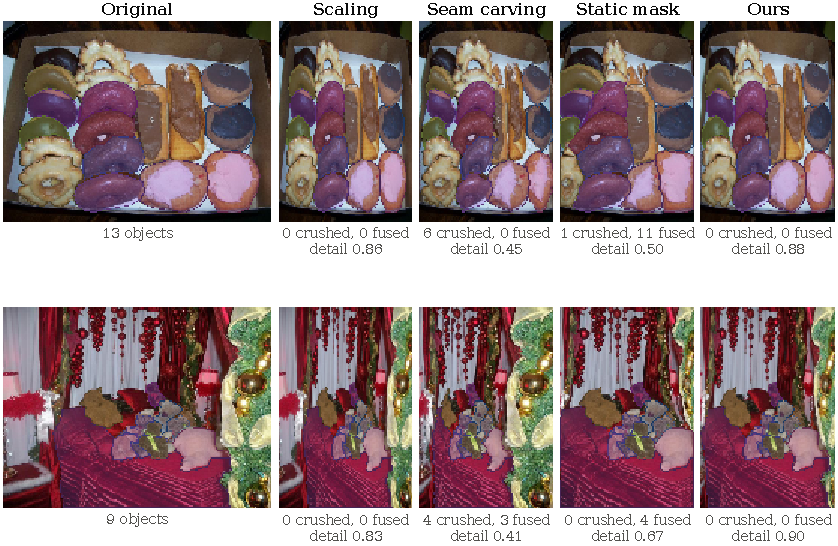
\includegraphics[width=\textwidth]{figs/coco.pdf}
\caption{Two COCO images (ground-truth objects tinted) resized to half width. Top: plain seam carving crushes 6 of 13 objects; the static mask fuses 11 and crushes 1. Bottom: seam carving crushes 4 objects and fuses 3; the static mask fuses 4. \ours{} damages none and keeps more detail than scaling. Carving does 19\% (top) and 61\% (bottom) of the resize before scaling takes over.}
\label{fig:coco}
\end{figure*}

\section{Evaluation Protocol}

All metrics are computed from the source map, so they are exact for carving and cropping and exact up to nearest-neighbour sampling for scaling. Let $A_k^0$ be the input area of object $k$, $A_k'$ its output area, and $\kappa_k$ the fraction of its input pixels that still appear in the output (scaling keeps all of them).
\begin{itemize}
\item \textbf{Crushed}: $\kappa_k < 0.5$. \textbf{Vanished}: $A_k' = 0$.
\item \textbf{Fused}: object $k$ is 4-adjacent to some object in the output that it was not adjacent to in the input.
\item \textbf{Intact}: not crushed, vanished or fused.
\item \textbf{Worse than scaling}: $A_k'/A_k^0$ is more than 2\% below the image's area ratio, i.e.\ the object shrank more than uniform scaling would have shrunk it.
\item \textbf{Squash} (aspect distortion): $|\log(a_k'/a_k)|$, where $a$ is the aspect ratio of the object's bounding box. Scaling to half width gives $\log 2 = 0.693$ for every object.
\item \textbf{Detail}: we crop the object's output bounding box, resize it back to its input bounding box, compute the SSIM map~\cite{wang2004ssim} ($7\times7$ windows, intensities in $[0,1]$) against the input crop, and average it over the object's own input pixels. Objects smaller than 7\,px in either dimension are not scored. \textbf{Detail lost}: detail $< 0.5$.
\item \textbf{Carved}: the share of the requested size change done by seams before any finishing step.
\end{itemize}
We deliberately do not report whole-image SSIM against the input: it requires equal sizes, and resizing the output back to the input size favours uniform scaling, which is exactly invertible up to blur. Per-object detail compares each object with itself, while squash measures the geometric distortion separately, so neither scaling nor carving gets a free advantage.

\section{Experiments}

\subsection{Setup}
We use the COCO128-seg subset of MS COCO~\cite{lin2014coco} with its ground-truth instance polygons. Objects covering less than 0.5\% of the image are dropped, and we keep the 70 images with at least three remaining objects (413 objects). Images are downscaled so their longer side is 320\,px, and each is resized to 75\% and 50\% of its width, the reductions used in RetargetMe. We run 18 configurations (2,520 runs in total), all on the same engine and all with forward energy unless stated otherwise. The classical fixes are: line protection, which adds a cost of 2 on long straight lines found with Canny edges~\cite{canny1986} and the probabilistic Hough transform~\cite{matas2000hough}; spectral-residual saliency~\cite{hou2007saliency} with weight 1; and a cost-knee stop that ends carving when the mean image-energy cost of the last 10 seams exceeds 2.5 times the median cost of the first 20, then scales the rest, in the spirit of~\cite{dong2009optimized}. Times are wall-clock seconds per image on one core of a 2-core cloud machine, in pure Python and NumPy. Re-running the full ablation reproduced every reported metric exactly.

\begin{table*}[t]
\centering
\caption{Ablation at 50\% width (70 images, 413 objects). ``Crushed'' includes vanished objects. Detail is mean per-object SSIM; squash is mean $|\log$ aspect change$|$ (lower is better). Rows below plain forward-energy seam carving add the named component to it.}
\label{tab:main}
\setlength{\tabcolsep}{3.5pt}
\begin{tabular}{lrrrrrrrrrr}
\toprule
Method & Intact\,\% & Crushed\,\% & Fused\,\% & Worse than & Images & Detail & Detail & Squash & Carved\,\% & s/img \\
 & $\uparrow$ & $\downarrow$ & $\downarrow$ & scaling\,\% $\downarrow$ & damaged\,\% $\downarrow$ & $\uparrow$ & lost\,\% $\downarrow$ & $\downarrow$ & & \\
\midrule
Uniform scaling & 97.1 & 0.0 & 2.9 & 1.2 & 9 & 0.865 & 0.0 & 0.693 & 0 & 0.00 \\
Centre crop & 57.6 & 42.4 & 0.0 & 41.4 & 86 & 0.410 & 63.7 & 0.361 & 0 & 0.00 \\
Seam carving, backward energy & 62.7 & 29.5 & 12.8 & 28.6 & 79 & 0.441 & 64.4 & 0.447 & 100 & 0.99 \\
Seam carving, forward energy & 64.9 & 29.5 & 8.5 & 28.3 & 84 & 0.461 & 58.8 & 0.500 & 100 & 0.93 \\
\midrule
\multicolumn{11}{l}{\emph{Classical fixes}} \\
\quad + line protection & 48.7 & 41.6 & 18.6 & 40.9 & 84 & 0.387 & 71.9 & 0.489 & 100 & 0.97 \\
\quad + saliency & 57.4 & 35.4 & 15.7 & 33.9 & 77 & 0.454 & 65.6 & 0.419 & 100 & 0.92 \\
\quad + cost-knee stop & 75.1 & 19.9 & 7.3 & 25.7 & 63 & 0.526 & 45.5 & 0.533 & 82 & 0.80 \\
\quad + all three & 64.4 & 25.7 & 14.5 & 30.0 & 70 & 0.530 & 51.3 & 0.477 & 79 & 0.76 \\
\midrule
\multicolumn{11}{l}{\emph{Object-aware}} \\
\quad + static object mask & 51.3 & 14.8 & 41.4 & 14.5 & 69 & 0.590 & 49.4 & 0.307 & 100 & 0.93 \\
\quad + per-object budget & 56.9 & 0.5 & 42.6 & 0.5 & 61 & 0.564 & 51.3 & 0.241 & 100 & 1.02 \\
\quad + budget + gap protection & 94.4 & 0.5 & 5.1 & 0.5 & 16 & 0.564 & 51.8 & 0.252 & 100 & 1.27 \\
\quad + guard, $\tau = 0.5$ & 99.0 & 0.0 & 1.0 & 0.5 & 3 & 0.571 & 50.4 & 0.263 & 98 & 1.35 \\
\quad + guard, $\tau = 0.2$ & 98.1 & 0.0 & 1.9 & 0.0 & 6 & 0.637 & 35.4 & 0.314 & 80 & 1.12 \\
\quad + guard, $\tau = 0.1$ & 98.5 & 0.0 & 1.5 & 1.2 & 4 & 0.728 & 16.9 & 0.360 & 63 & 0.90 \\
\quad + guard, $\tau = 0.05$ & 97.6 & 0.0 & 2.4 & 1.0 & 6 & 0.792 & 9.2 & 0.386 & 54 & 0.78 \\
\quad \best{+ guard, $\tau = 0$ (\ours{})} & \best{99.0} & \best{0.0} & \best{1.0} & \best{0.0} & \best{3} & \best{0.911} & \best{0.2} & \best{0.464} & \best{37} & \best{0.53} \\
\midrule
\ours{}, crop finish & 68.0 & 32.0 & 0.0 & 31.7 & 69 & 0.522 & 53.3 & 0.223 & 37 & 0.54 \\
\ours{} + lines + saliency & 97.6 & 0.0 & 2.4 & 0.2 & 7 & 0.897 & 0.2 & 0.573 & 20 & 0.31 \\
\bottomrule
\end{tabular}
\end{table*}


\subsection{Classical fixes do not protect objects}
Table~\ref{tab:main} shows that plain forward-energy carving leaves only 64.9\% of objects intact at half width: 29.5\% are crushed and 8.5\% fused, and 84\% of images contain at least one damaged object. Forward energy improves on backward energy mainly by fusing fewer objects. Line protection and saliency make integrity \emph{worse} (48.7\% and 57.4\% intact). Our hypothesis is that both fixes raise the cost of background structure (straight lines in COCO are mostly tables, walls and markings, and spectral-residual saliency often highlights background clutter), leaving fewer cheap background paths, so the cheapest seam crosses an object more often. We have not yet verified this; measuring the share of seam pixels inside objects with and without each fix would test it. The cost-knee stop helps (75.1\% intact), mainly by stopping early and letting scaling do 18\% of the resize.

\subsection{Static masks trade crushing for fusion}
Adding a static object mask lowers crushing from 29.5\% to 14.8\% but raises fusion from 8.5\% to 41.4\%, so the share of intact objects \emph{falls} to 51.3\%. When objects are expensive, seams move into the strips between them. The per-object budget removes almost all crushing (0.5\%) but still fuses 42.6\% of objects. Gap protection is the component that addresses fusion: with budget and gaps, and no guard, 94.4\% of objects are intact. These numbers are measured, not enforced, and show that the cost terms do most of the work. The guard closes the remaining cases (99.0\% intact); the remaining 1.0\% of fused objects come from the scaling finish, which can remove a 1-px gap between objects (uniform scaling alone fuses 2.9\%).

\subsection{Integrity is not enough: the dial}
At $\tau = 0.5$ the guard keeps 99.0\% of objects intact, yet half of all objects (50.4\%) lose their detail, because seams still pass through them and shift their texture and outline. We first noticed this on the coins photo (Fig.~\ref{fig:coins}), where every coin survived as a separate shape but its face was distorted, and it motivated the detail metric. Lowering $\tau$ trades squash for detail monotonically (Fig.~\ref{fig:dial}). At $\tau = 0$, detail rises to 0.911 and detail lost falls to 0.2\%. Compared with uniform scaling, \ours{} keeps more detail (0.911 vs.\ 0.865) and squashes objects less (0.464 vs.\ 0.693); compared with plain seam carving, it is better on every integrity and detail measure. It is also faster than plain carving (0.53\,s vs.\ 0.93\,s), because it stops early and scaling is nearly free.

The gain over scaling has a simple explanation. At half width, carving removes on average 37\% of the width reduction from background, about $0.185W$, so the remaining $0.815W$ is scaled to $0.5W$. Objects are therefore scaled by about 0.61 instead of 0.5, a squash of $\log(1/0.61)\approx 0.49$, close to the measured mean of 0.464.

\begin{figure}[t]
\centering
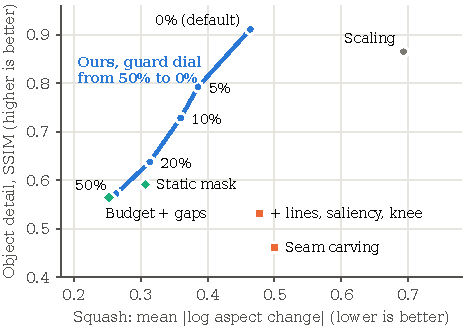
\includegraphics[width=\columnwidth]{figs/dial.pdf}
\caption{Per-object detail against squash at half width. Lowering the guard dial $\tau$ from 50\% to 0\% moves \ours{} from the region of the static mask and budget-plus-gaps configurations (no guard) to a point that improves on uniform scaling in both detail and squash. Plain seam carving and the classical fixes are worse on both axes than every object-aware configuration.}
\label{fig:dial}
\end{figure}


\subsection{Moderate resizing and finishing step}
At 75\% width all methods do better, but the ranking holds. Plain forward-energy carving keeps 93.9\% of objects intact with detail 0.656; static masks keep 77.0\% (21.8\% fused); budget with gaps keeps 100\%, but with detail 0.772. \ours{} keeps 99.0\% intact with detail 0.963 and squash 0.135, against 0.932 and 0.286 for uniform scaling, and carving does 54\% of the resize. Replacing the scaling finish with an object-aware crop is clearly worse at half width (68.0\% intact), because a crop must cut objects near the image border. Adding line and saliency costs on top of our method stops carving earlier (20\% carved) and slightly lowers both detail and squash quality, consistent with the negative results above. Fig.~\ref{fig:coco} shows two COCO examples.

\section{Limitations}

\textbf{The guard enforces part of the result.} ``0\% crushed'' for \ours{} holds by construction. The evidence that the method works is in the quantities the guard does not control: budget plus gaps without a guard (94.4\% intact), the detail score, which exposed the failure of $\tau = 0.5$, and the share of the resize that carving still performs.

\textbf{Carving often stops early.} At half width, carving does 37\% of the resize on average (median 29\%), and in 16\% of the images it stops before the first seam, so the result equals uniform scaling. On crowded images the method is never worse than scaling on objects, but it is not much better.

\textbf{The budget is inactive at the default.} At $\tau = 0$ no object loses pixels, so the exponential budget reduces to a static mask; the components that matter at the default are gap protection and the guard.

\textbf{Data and masks.} We use 70 images and ground-truth masks at 320\,px, which is enough to separate large effects but not small ones; for example, we do not claim that 99.0\% vs.\ 97.1\% intact (ours vs.\ scaling) is significant, and we have not yet computed confidence intervals. Objects under 0.5\% of the image are unprotected. A detector will miss objects, which are then treated as background. Height reduction and enlarging are implemented but not evaluated.

\textbf{The detail metric is not yet validated against people.} It agrees with what we see in our examples, but a user study is needed to confirm that it predicts preference. We have also not evaluated against learning-based methods~\cite{shen2024prune,elsner2024deformation}.

\textbf{Greedy carving.} Each seam is optimal on its own, but the sequence of seams is greedy, and the guard stops at the first refused seam even if a later seam would have been safe. The parameters $\gamma$, $\mu$ and $g$ were set by reasoning, not tuned.

\section{Conclusion and Future Work}

Seam carving and its common fixes silently crush and fuse objects, and existing evaluations do not measure it. With exact pixel correspondences we count object damage directly and score per-object detail, and we show that a static object mask, the standard remedy, mostly converts crushing into fusion. Gap protection and an exact integrity guard remove both failures, and setting the guard to admit only background seams yields a resize that is better than uniform scaling in both object detail and squash, with no training and on a CPU. Next steps are a full-scale evaluation on COCO val2017 and RetargetMe with predicted masks and confidence intervals, a paired user study following the RetargetMe protocol to validate the detail metric, choosing $\tau$ per image or per object class, and a comparison with learning-based retargeting under the same object-integrity metrics.

\bibliographystyle{IEEEtran}
\bibliography{refs}

\end{document}
